\documentclass[11pt]{article}


\usepackage[top=2cm, bottom=2cm, left=3.5cm, right=3.5cm]{geometry}
\usepackage{hyperref}       % hyperlinks
\usepackage{url}            % simple URL typesetting
\usepackage{booktabs}       % professional-quality tables
\usepackage{microtype}      % microtypography
\usepackage[table, dvipsnames, svgnames]{xcolor}  % colors
\usepackage[outline]{contour}% http://ctan.org/pkg/contour
\usepackage{wrapfig}
\usepackage{graphicx}
\usepackage{bm}
\usepackage{bbm}
\usepackage{multirow}
\usepackage{pifont}
\usepackage{rotating}
\usepackage{tikz}
\usepackage{amsmath}
\usepackage{amsfonts}
\newcommand{\xmark}{\ding{55}}%

\setlength{\tabcolsep}{3.5pt}

\hypersetup{
	colorlinks=true, %set true if you want colored links
	linktoc=all,     %set to all if you want both sections and subsections linked
	linkcolor=black,  %choose some color if you want links to stand out
	citecolor=cyan,
}




\allowdisplaybreaks



\newcommand{\defeq}{\vcentcolon=}
\newcommand{\im}{\operatorname{im}}
\newcommand{\Hom}{{\rm{Hom}}}
\newcommand{\diam}{{\rm{diam}}}
\newcommand{\dom}{\text{dom}}
\newcommand{\ovl}{\overline}
\newcommand{\rr}{\mathbb{R}}
\newcommand{\EE}{\mathcal{E}}
\newcommand{\VV}{\mathcal{V}}
\newcommand{\mystar}{{\fontfamily{lmr}\selectfont$\star$}}
\newcommand{\llangle}{\langle \langle}
\newcommand{\rrangle}{\rangle \rangle}

%bold commands
\newcommand{\xx}{\bm{x}}
\newcommand{\Xx}{\bm{X}}
\newcommand{\Tt}{\bm{T}}
\newcommand{\yy}{\bm{y}}
\newcommand{\ee}{\bm{e}}
\newcommand{\cc}{\bm{c}}
\newcommand{\uu}{\bm{u}}
\newcommand{\vv}{\bm{v}}
\newcommand{\ww}{\bm{w}}
\newcommand{\om}{\bm{\omega}}
\newcommand{\al}{\bm{\alpha}}
\newcommand{\be}{\bm{\beta}}
\newcommand{\si}{\bm{\sigma}}
\newcommand{\ta}{\bm{\tau}}


%calcommand

\newcommand{\mc}{\mathcal}

\DeclareMathOperator*{\argmax}{arg\,max}
\DeclareMathOperator*{\argmin}{arg\,min}

\setlength{\parindent}{0pt}

\author{Simone Manti, AU ID 734894, \texttt{smanti@mpe.au.dk} \\
	Final project for Neural Networks and Deep Learning 2024}

\title{Symbolic Model-Based Reinforcement Learning}



\begin{document}
	\maketitle

\section{Introduction}

\section{Model-Based Reinforcement Learning}
Reinforcement Learning (RL), contrarily to standard Supervised Learning, requires a continue interaction with data to update the policy. Usually, model-free RL is employed to optimize the policy, where the agent can only use the data sampled interacting with the real environment. In particular, RL algorithms with high sample complexity are non-manageable in a real-world scenario due to its computational cost. An alternative is presented by the so-called Model-Based Reinforcement Learning (MBRL) \cite{moerland2023model}, where apart from optimizing policy the environment model must be learned. In real-world scenario, having an environment model drastically reduces the complexity of generating new training samples for RL algorithms.
In the following, we briefly overview the main components of MBRL. A more extensive treatment can be found in \cite{moerland2023model, pineda2021mbrl,luo2024survey}. 

MBRL restates the problem as a Markov Decision Process (MDP) \cite{puterman2014}. A MDP is a tuple $\{\mathcal{S}, \mathcal{A}, \mathcal{T}, \mathcal{R}, p(s_0), \gamma\}$, where $\mathcal{S}$ and $\mathcal{A}$ are, respectively, the state and the action space, $\mathcal{T}: \mathcal{S} \times \mathcal{A} \rightarrow p(\mathcal{S})$ is the \textsl{transition function}, $\mathcal{R}: \mathcal{S} \times \mathcal{A} \times \mathcal{S} \rightarrow \rr$ is the \textsl{reward function}, $p(s_0)$ is the initial state distribution and $\gamma \in [0,1]$ is a discount parameter.
A solution to a finite-time MDP consists of a policy $\pi^*: \mathcal{S} \rightarrow \mathcal{A}$ which maximizes the expected sum of rewards, that is
\begin{equation}
	\pi^* = \argmax_{\pi} Q^{\pi}(s,a) = \argmax_{\pi} \mathbb{E}_{\pi, \mathcal{T}}\left[\sum_{k=0}^K \gamma^k r_{t+k} | s_t = s, a_t = a \right], \label{eq: expected_sum_rewards}
\end{equation}

where $s_t \in \mathcal{S}, a_t \in \mathcal{A}, r_t := \mathcal{R}(s_t, a_t, s_{t+1})$.

MBRL approaches repeat the following two steps iteratively:
\begin{enumerate}
	\item collect (or enlarge the current data with) a dataset $\mathcal{D} := \{(s_i, a_i, s_{i+1}, r_i, d_i)\}_{i=1}^N$, where $d_i$ is the termination value indicating the end of the episode, and learn an approximate model $f^*$ of the environment's dynamics fitting $\mathcal{D}$, \textsl{i.e.}
	\begin{equation}
		f^* = \argmax_{f \in \mathcal{F}} \mathbb{E}_{(s_t, a_t, s_{t+1}) \sim \mathcal{D}} \mathcal{L}(s_{t+1}, f(s_t, a_t)),
	\end{equation}
	where $\mathcal{F}$ is a general family of functions (for instance Neural Networks) and $\mathcal{L}$ is a loss function. Note that with the same data reward and termination functions can be learned reward as well;
	\item simulate the transition with the learned model $f^*$ and optimize the policy maximizing the expected sum of rewards like in \eqref{eq: expected_sum_rewards}.
\end{enumerate}

\section{Symbolic Regression}
SR consists of finding a mathematical expressions that best fits a given dataset without assuming a particular structure of the expression. 
In our case, SR is handled with Genetic Programming (GP) \cite{koza1994genetic, o2009riccardo}. GP is an evolutionary strategy that explores a space of candidate models/functions by iteratively updating an initial population through genetic operations. A candidate model is also called \textsl{individual} and can be easily represented by a tree, in which each node is either a \textsl{primitive} (\textsl{i.e.} an operator) or a \textsl{terminal} (\textsl{i.e.} a variable or constant).
\paragraph{Initialization} The population is typically initialized randomly. Some well-known techniques are the \textsl{full} and the \textsl{grow} method (see Section 2.1 in \cite{o2009riccardo}), and a combination of those gives rise to \textsl{ramped half and half}. Each of them assumes that the starting population contains individuals that do not exceed a fixed maximum depth.

\paragraph{Selection} Usually genetic operations are performed on individuals that are selected based on fitness, \textsl{i.e.} that are ``probably good''. One way to do so is \textsl{tournament selection}. This consists of performing a tournament for each $k$ (tournament size) individuals, competing in terms of their fitnesses. The higher the score in these tournaments, the higher the probability for these individuals to be chosen. In our method, $k=2$ and we assign a non-zero probability to pick the loser instead of the winner in each tournament. This is calibrated in the hyperparameter selection phase. 

\paragraph{Crossover and Mutation} Genetic operations consists of \textsl{crossover} and \textsl{mutation}. The most common crossover used is the \textsl{subtree crossover} (or \textsl{one-point crossover}): given two parent trees, a random subtree and a crossover point are chosen for both; then, two new trees are generated, named \textsl{offsprings}, replacing the subtree rooted in the first parent with the one in the second parent and vice-versa.
Instead, the most common mutation creates an offspring for a given parent tree by replacing a (randomly chosen) subtree with a newly generated subtree. 

\section{Experiments and implementations details}
\textcolor{red}{Add intro + libraries used}


\subsection{Simple 1-dimensional MDP}
\label{sec: simple_1_dmdp}
The following simple 1-dimensional MDP, with episode length 10, is considered
\begin{align}
	&s_{t+1} := s_t + a_t, \label{eq: simple_1dmpd_dynamics}\\ 
	&r_t := \cos(2\pi s_{t+1})\exp(|s_{t+1}|/3). \label{eq: simple_1dmpd_reward}
\end{align}

In this case, the goal is learning both the dynamics eq.~\eqref{eq: simple_1dmpd_dynamics} and the reward function eq.~\eqref{eq: simple_1dmpd_reward}. \textcolor{red}{add details on training data used}

\paragraph{SR hyperparameters} The following hyperparameters are used: 10 optimizer iterations, population size 5000, 10000 generations, \texttt{add,sub,mul,div,constant,variable,} \texttt{sin,exp,abs} as allowed symbols and 32 threads. Note that to complicate the problem \texttt{cos} is not in the primitive set.

\paragraph{NN hyperparameters} A standard Multi-Layer Perceptron (MLP) is considered with the following hyperparameters: 4 hidden layers with 200 nodes each, SiLU activation function, Adam optimizer with 2000 epochs, batch size 256, patience epochs 25, learning rate $7.5e-4$ and weight decay $3e-5$.

\paragraph{Results} Figure~\ref{fig: simple_1dmdp} demonstrates that SR learned solution generalizes better outside the training region, while the NN model overfits in the training distribution. SR learned the following models (rounded to the first $3$ decimal digits):
\begin{align}
	&s_{t+1} = 1.0s_t + 1.0a_t, \label{eq: sr_simple_1dmdp_dynamics}\\
	&r_t = 1.0\exp(|0.333s_{t+1}|)\sin(6.283s_{t+1} - |-0.023 s_t + \sin(0.023 s_t) + 1.571|).\label{eq: sr_simple_1dmdp_reward}
\end{align}

Note that eq.~\eqref{eq: simple_1dmpd_dynamics} coincides with eq.~\eqref{eq: simple_1dmpd_dynamics}, while eq.~\eqref{eq: sr_simple_1dmdp_reward} is slightly different than eq.~\eqref{eq: simple_1dmpd_reward}. However, the first of the two factors matches completely with the ground truth, while the latter is approximately $\sin(2\pi s_{t+1} + 1.571)$ using that $6.283\approx 2\pi$ and that $sin(x) \approx x$ for $x>0$ sufficiently small. A similar model for the reward function was also found in the original paper \cite{kamienny2022symbolic}.

\begin{figure}
	\centering
	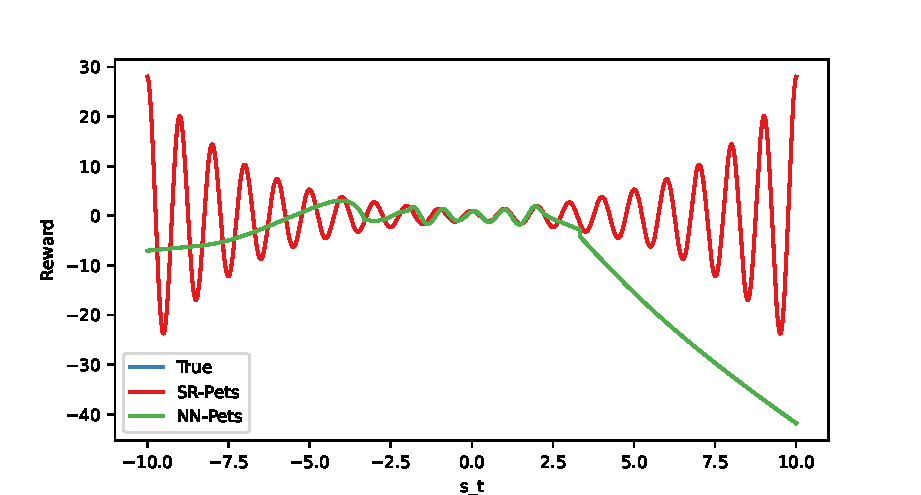
\includegraphics{simple1dmdp_pets.pdf}
	\caption{Reward function, evaluated with $a_t=0$, predicted by the learned models}
	\label{fig: simple_1dmdp}
\end{figure}

\subsection{Cartpole}

\begin{align}
	&\ddot{\theta} = \frac{g\sin(\theta) + \cos(\theta)\left(\frac{-K_{\rm mag} a - m_p l \dot{\theta}^2\sin(\theta)}{m_c + m_p}\right)}{l\left(\frac{4}{3} - \frac{m_p\cos^2(\theta)}{m_c+m_p}\right)}\\
	& \ddot{x} = \frac{K_{\rm mag} a + m_pl(\dot{\theta}^2\sin(\theta) - \ddot{\theta}\cos(\theta))}{m_c + m_p}
\end{align}


\paragraph{SR hyperparameters} As in \ref{sec: simple_1_dmdp} but with allowed symbols \texttt{add,sub,mul,div,constant,} \texttt{variable,sin,cos,pow}.

\paragraph{NN hyperparameters} As in \ref{sec: simple_1_dmdp}.

\paragraph{Results}


\section{Conclusion and discussion}


\bibliographystyle{ieeetr}
\begin{thebibliography}{10}
	\bibitem{kamienny2022symbolic}
	P.A.~Kamienny, S.~Lamprier, ``Symbolic-Model-Based Reinforcement Learning''.
	{\em NeurIPS 2022 AI for Science: Progress and Promises}, 2022.
	
	\bibitem{puterman2014}
	M. L.~Puterman, ``Markov Decision Processes: Discrete Stochastic Dynamic Pro-
	gramming.'' {\em John Wiley and sons}, 2014.
	
	\bibitem{moerland2023model}
	T.M.~Moerland, J.~Broekens, A.~Plaat, C.M.~Jonker, ``Model-based Reinforcement Learning: A Survey''. {\em Foundations and Trends in Machine Learning}, 2023.
	
	\bibitem{pineda2021mbrl}
	L.~Pineda, B.~Amos, A.~Zhang, N.O~Lambert, R.~Calandra, ``Mbrl-lib: A Modular Library for Model-Based Reinforcement Learning''. {\em arXiv preprint arXiv:2104.10159}, 2021.
	
	\bibitem{luo2024survey}
	F.~Luo, T.~Xu, H.~Lai, X.~Chen, W.~Zhang, Y.~Yu, ``A Survey on Model-Based Reinforcement Learning''. {\em Science China Information Sciences}, 2024.
	
	\bibitem{koza1994genetic}
	J.R.~Koza, ``Genetic programming as a means for programming computers by natural selection'', 
	{\em Statistics and Computing}, vol.~4, 1994.
	
	\bibitem{o2009riccardo}
	R.~Poli et al., ``A Field Guide to Genetic Programming''.
	\newblock Published via \texttt{http://lulu.com} and freely available at \texttt{http://www.gp-field-guide.org.uk}, 2008.
	
\end{thebibliography}
\end{document}